\subsection{Sensores en General}

\par
Un sensor es un dispositivo capaz de detectar magnitudes físicas o químicas, llamadas variables de instrumentación, y transformarlas en variables eléctricas.

\begin{itemize}
	\item Las variables de instrumentación pueden ser por ejemplo: temperatura, intensidad lumínica, distancia, aceleración, inclinación, desplazamiento, presión, fuerza, torsión, humedad, movimiento, pH, etc.
	
	\item Una variable eléctrica puede ser una resistencia eléctrica (como en una RTD), una capacidad eléctrica (como en un sensor de humedad o un sensor capacitivo), una tensión eléctrica (como en un termopar), una corriente eléctrica (como en un fototransistor), etc.
\end{itemize}

\par \noindent
Los sensores se pueden clasificar en función de los datos de salida en: digitales y analógicos\cite{sensores-arduino}.

\subsubsection{Características de los Sensores \cite{sensores-wiki}}

\begin{itemize}
	
	\item Rango de medida: dominio en la magnitud medida en el que puede aplicarse el sensor.
	
	\item Precisión: es el error de medida máximo esperado.
	
	\item Offset o desviación de cero:  valor de la variable de salida cuando la variable de entrada es nula. Si el rango de medida no llega a valores nulos de la variable de entrada, habitualmente se establece otro punto de referencia para definir el offset.
	
	\item Linealidad o correlación lineal.
	
	\item Sensibilidad de un sensor: suponiendo que es de entrada a salida y la variación de la magnitud de entrada.
	
	\item Resolución: mínima variación de la magnitud de entrada que puede detectarse a la salida.
	
	\item Rapidez de respuesta: puede ser un tiempo fijo o depender de cuánto varíe la magnitud a medir. Depende de la capacidad del sistema para seguir las variaciones de la magnitud de entrada.
	
	\item Derivas: son otras magnitudes, aparte de la medida como magnitud de entrada, que influyen en la variable de salida. Por ejemplo, pueden ser condiciones ambientales, como la humedad, la temperatura u otras como el envejecimiento (oxidación, desgaste, etc.) del sensor.
	
	\item Repetitividad: error esperado al repetir varias veces la misma medida.
	
\end{itemize}

\par \noindent
Debido a que solamente la magnitud física que nos interesa para nuestro proyecto es la temperatura. Tomamos encuenta los posibles candidatos para utilizar como sensor de temperatura en el prototipo.

\clearpage

\subsubsection{Sensores de Temperatura}	

\paragraph{DS18B20}
El termómetro digital DS18B20 proporciona de 9 bits a 12 bits.
Mediciones de temperatura en grados celsius y tiene una función de alarma no volátil programable por el usuario. El DS18B20 se comunica a través de un Bus de 1 cable que por definición requiere solo una línea de datos (y tierra) para la comunicación con un microprocesador central. Además, el DS18B20 puede obtener potencia directamente desde la línea de datos, eliminando la necesidad de una fuente de alimentación externa\cite{ds18b20}.

\begin{figure}[H]
	\centering
	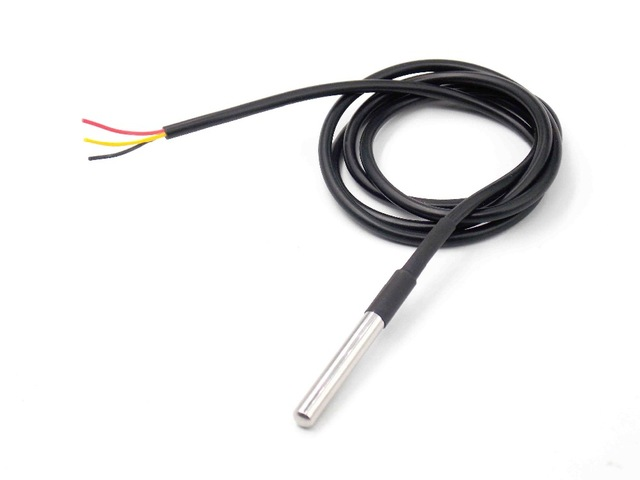
\includegraphics[width=0.5\textwidth]{sensores1.jpg}
	\caption{Sensor DS18B20 estilo sonda}
\end{figure}

\par \noindent
Mide las temperaturas de -55 ° C a 125 ° C, ± 0.5 ° C de  precisión entre -10 ° C a + 85 ° C y resolución programable de 9 a 12 bits.

\par \noindent
Las aplicaciones que pueden beneficiarse de esta característica incluyen
Controles ambientales, monitoreo de temperatura
sistemas dentro de edificios, equipos o maquinaria, y
sistemas de monitoreo y control de procesos\cite{ds18b20}. 


\paragraph{DHT11}
El sensor digital de temperatura y humedad DHT11 es un sensor compuesto que contiene una
señal digital de salida de la temperatura y la humedad. Aplicación de módulos digitales dedicados
tecnología de recolección y la tecnología de detección de temperatura y humedad, para asegurar que
el producto tiene una alta fiabilidad y una excelente estabilidad a largo plazo. El sensor incluye un sentido resistivo
de componentes húmedos y dispositivos de medición de temperatura NTC, y conectado con un
microcontrolador de alto rendimiento de 8 bits\cite{dht11}.

\begin{figure}[H]
	\centering
	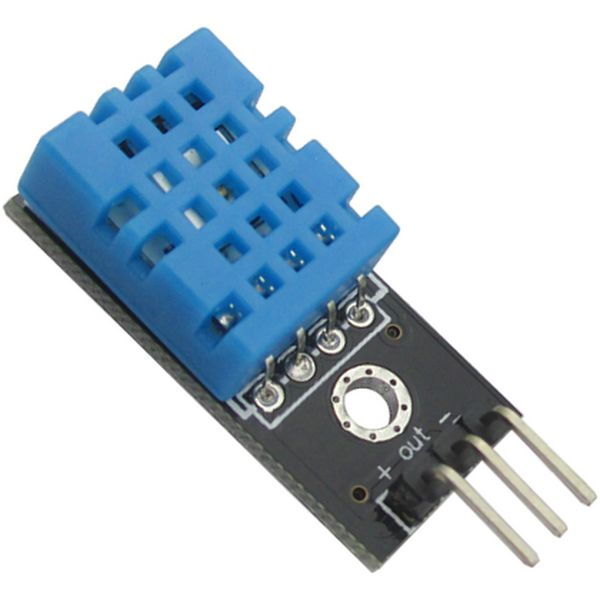
\includegraphics[width=0.25\textwidth]{sensores2.jpg}
	\caption{Sensor DHT11 en placa}
\end{figure}

\par \noindent
Mide temperaturas de 0 ° C a 50 ° C con una precisión de ±2 ° C en 25 ° C y una resoluación no programable de 16 bits.

\par \noindent
Aplicaciones de este sensor son principalmente para mediciones de humedad y temperatura relativa. Donde se require obtener valores en ambas magnitudes y no tanta precisión de una magnitud en particular\cite{dht11}. 

\par \noindent
Los sensores de temperatura y la plataforma de Arduino nos permite crear un prototipo de medición de temperatura; sin embargo, aun no es un termómetro como tal y mucho menos uno que SIGCSA pueda utilizar en campo. Hay que definir el concepto de termómetro para aplicarlo en nuestro prototipo.

